\chapter{Studi Literatur}

Bab Studi Literatur digunakan untuk mendeskripsikan kajian literatur yang terkait dengan persoalan tugas akhir. Tujuan studi literatur adalah:

\begin{enumerate}
  \item menunjukkan kepada pembaca adanya gap seperti pada rumusan masalah yang memang belum terselesaikan,
  \item memberikan pemahaman yang secukupnya kepada pembaca tentang teori atau pekerjaan terkait yang terkait langsung dengan penyelesaian persoalan, serta
  \item menyampaikan informasi apa saja yang sudah ditulis/dilaporkan oleh pihak lain (peneliti/Tugas Akhir/Tesis) tentang hasil penelitian/pekerjaan mereka yang sama atau mirip kaitannya dengan persoalan tugas akhir.
\end{enumerate}

\blindtext

\blindtext

\section{Intrusion Detection}

  \subsection{Definisi Umum}

  Deteksi intrusi adalah suatu proses memantau setiap kejadian yang muncul pada sistem atau jaringan dan menganalisanya untuk menemukan tanda akan adanya insiden yang terjadi. Insiden bisa berupa pelanggaran kebijakan keamanan komputer, kebijakan penggunaan yang diterima, atau praktek keamanan standar.

  Insiden dapat diakibatkan oleh banyak hal, seperti malware, penyerang dari luar yang tidak berhak mengakses sistem, dan pengguna yang menyalahi kebijakan keamanan.

  Deteksi intrusi berfokus utama pada mengidentifikasi kemungkinan insiden, mencatat informasi terhadap insiden tersebut, dan melaporkan insiden kepada pengelola keamanan sistem.

\section{Intrusion Detection System}

  \subsection{Definisi Umum}

  Sistem deteksi intrusi adalah perangkat lunak yang mengotomasi proses deteksi intrusi. Sistem mengambil paket yang masuk sambil melakukan analisis.  \\

  \subsection{Metodologi Deteksi}

  Ada empat macam metode deteksi yang biasa dipakai dalam sistem deteksi intrusi.

    \subsubsection{Signature-based Detection}

    Signature adalah pola yang berkaitan dengan ancaman yang dikenal. Deteksi berbasis signature adalah proses membandingkan signature dengan aktivitas sistem untuk mengidentifikasi insiden yang mungkin. Contoh signature yaitu: 

    \begin{enumerate}
      \item Usaha melakukan akses melalui telnet dengan username “root”, yang menyalahi kebijakan keamanan organisasi
      \item Email dengan subyek “Free pictures” dan lampiran dengan nama “freepics.exe”, adalah karakteristik dari malware
      \item System log entry dari sistem operasi dengan kode status 645, yang mengindikasikan host auditing sedang mati
    \end{enumerate}
    

    Pengenalan berbasis signature sangat efektif untuk mendeteksi ancaman yang telah dikenal tapi tidak efektif untuk mendeteksi ancaman yang belum dikenal sebelumnya atau ancaman yang disamarkan dengan teknik-teknik tertentu.

    Metode ini adalah metode termudah karena hanya membandingkan unit aktivitas saat ini, seperti paket atau log entry, pada daftar signature menggunakan operasi perbandingan string. Metode berbasis signature membutuhkan sedikit pengetahuan tentang protokol jaringan dan aplikasi, dan tidak dapat melacak atau mendapat state dari komunikasi yang kompleks.

    \subsubsection{Anomaly-based Detection}

    Deteksi dengan anomali adalah proses membandingkan parameter aktivitas yang dianggap normal dengan aktivitas sistem sekarang untuk melihat penyimpangan yang signifikan. Sistem menggunakan profile untuk menentukan parameter aktivitas normal seperti user, host, koneksi jaringan, atau aplikasi. Profil dikembangkan dengan memantau karakteristik dari aktivitas sejenis selama selang waktu tertentu.

    Sistem akan menggunakan metode statistik untuk membandingkan karakteristik aktivitas sekarang terhadap batas yang terkait dengan profile. Ketika ada aktivitas yang menyimpang cukup jauh dari batas, akan dicatat ke log dan dilaporkan ke pengelola. Profil bisa dikembangkan dari berbagai atribut, seperti jumlah email yang dikirim oleh pengguna, jumlah percobaan login yang gagal, dan tingkat penggunaan CPU host waktu tertentu.

    Keuntungan dari metode berbasis anomali ini adalah dapat mendeteksi ancaman yang belum pernah dikenal sebelumnya. Contoh, sebuah komputer terinfeksi dengan sebuah malware yang menggunakan resource dalam jumlah besar, mengirim banyak email, menjalankan banyak koneksi, dan melakukan kegiatan lain yang cukup berbeda dari profile sistem normal.

    Profile awal dibangkitkan selama rentang waktu tertentu yang disebut training period. Profile bisa statis atau dinamis. Dinamis ketika profile diperbaharui dengan log aktivitas sistem. Statis jika profile diperbaharui secara manual.

    \subsubsection{Stateful Protocol Analysis}

    % \blindtext

  \subsection{Tipe Teknologi Network Intrusion Detection System}

  \subsection{Teknologi Network Intrusion Detection System}
    \subsubsection{SNORT IDS}

\section{Dasar Teori}
Perujukan literatur dapat dilakukan dengan menambahkan entri baru di berkas. Tulisan ini merujuk pada \parencite{knuth2001art} dan \parencite{4026885}

  \subsection{Subbab}

  \blindtext

  \begin{figure}[h]
    \centering
    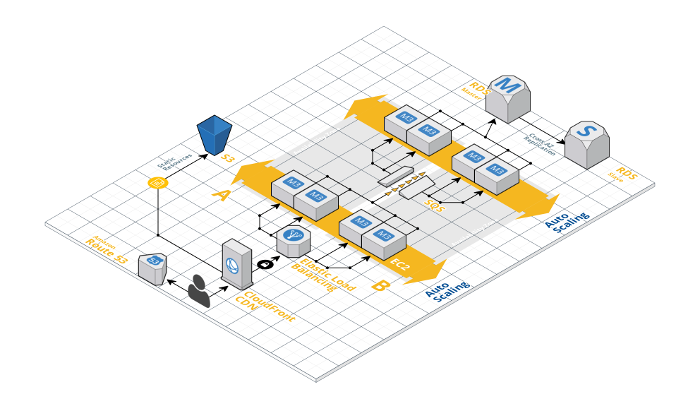
\includegraphics[width=0.8\textwidth]{resources/chapter-2-infrastructure-diagram.png}
    \caption{Contoh gambar}
  \end{figure}

  \subsubsection{Subsubbab}

  \blindtext

\section{Studi Terkait}
\blindtext
